\documentclass[12pt]{article}
\usepackage[a4paper, total={6in, 8in}]{geometry}
\usepackage{tikz}

\usetikzlibrary{automata,shapes.multipart}

\begin{document}
	\section*{Entwurfsskizze}

	Das Programm ist aufgeteilt in Frontend und Backend. Das Frontend ist verantwortlich für das GUI und Events (Mausklicks, Knopfdrücke, etc.),
	sowie für das graphische Darstellen der Daten aus dem Backend.
	Das Backend ist verantwortlich für das Parsing des Inputs sowie für die Vorbereitung der Daten für das Frontend.

	\subsection*{Backend}
	%\begin{figure}[h!]
	%	\begin{center}
	%		\begin{tikzpicture}[%
	%				every node/.style={%
	%					align=left,
	%					state,
	%					rectangle split,
	%					rectangle split parts=3
	%				}    
	%			]
	%
	%			\node (function) at (0, 0) {%
	%				\textbf{Function}
	%
	%				\nodepart{second}
	%				+\texttt{at()} \\
	%				+\texttt{isValid(): boolean} \\
	%				+\texttt{setDomain()} \\
	%				+\texttt{getDomain(): Interval} \\
	%				+\texttt{getRange(): Interval} \\
	%				+\texttt{getRoots(): ArrayList<Double>} \\
	%				+\texttt{getExtrema(): ArrayList<Double>} \\
	%				+\texttt{getInflections(): ArrayList<Double>} \\
	%				+\texttt{getPoles(): ArrayList<Double>}\\
	%				+\texttt{getSyntaxError(): SyntaxError}
	%
	%				\nodepart{third}
	%				-\texttt{test(): float}
	%			};

				% \node (parser) [draw] at (0, -2) {Parser};
	%		\end{tikzpicture}
	%	\end{center}
	%	\caption{Test}
	%\end{figure}

	Das Backend stellt dem GUI die Klasse \texttt{Function} zum Abfragen der Daten und Metadaten einer Funktion zur verfügung.
	Darüber hinaus beinhaltet \texttt{Function} ein Objekt der Klasse \texttt{Parser}, welche in der Lage ist einen Term (gegeben als \texttt{String}) in einen
	Expression Tree umzuwandeln.

	Es gibt eine abstrakte Klasse \texttt{INode} welche eine generische Node im Expression Tree repräsentiert.
	\begin{figure}[h!]
		\begin{center}
			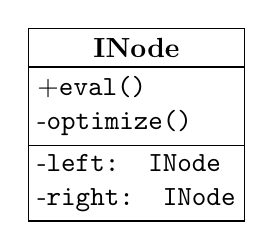
\begin{tikzpicture}[%
					every node/.style={%
						align=left,
						state,
						rectangle split,
						rectangle split parts=3,
						rectangle split part align = {center, left, left}
					}    
				]
	
				\node (function) at (0, 0) {%
					\textbf{INode}
	
					\nodepart{second}
					+\texttt{eval()} \\
					-\texttt{optimize()}
	
					\nodepart{third}
					-\texttt{left: INode} \\
					-\texttt{right: INode}
				};

				% \node (parser) [draw] at (0, -2) {Parser};
			\end{tikzpicture}
		\end{center}
		\caption{Klassenstruktur der Klasse \texttt{INode}}
	\end{figure}
	Wie gewohnt verweisen \texttt{left} und \texttt{right} auf die entsprechenden Unterbäume, und \texttt{eval()} wertet die Node (an einer gegebenen Stelle) aus.
	Dabei werden die \texttt{eval()} Funktionen der Unterbäume aufgerufen und mit der entsprechenden Operation miteinander verrechnet. 
	Jede unterstützte Operation (inklusive Konstanten, Variablen und Schlüsselwörtern) sind eigene Klassen welche von \texttt{INode} erben.

	Die \texttt{optimize()} Funktion optimiert den Expression Tree indem er konstante Ausdrücke bereits ausrechnet und vereinfacht. D.h. gibt man zum Beispiel \texttt{3+5} ein, so wird
	der Expression Tree zu einer einzelnen Node vom Typ \texttt{Rational} mit Wert \texttt{8} reduziert.

	Die \texttt{Function} Klasse besitzt den Parser um die Funktion an einer gegeben Stelle auszuwerten. Desweiteren analysiert sie die Funktion in einem
	gegebenen Definitionsbereich auf Nullstellen, Extremstellen, Wendestellen und Polstellen. Diese Stellen werden dem GUI ebenfalls
	zur Verfügung gestellt. Zudem ermittelt die Klasse den Wertebereich der Funktion in dem gegebenen Definitionsbereich.

	\subsection*{Frontend}
	Das Frontend besteht aus zwei Klassen; GUI behinhaltet die Formatierung des Fensters und besteht aus einem JFrame und mehreren JPanels.
	Wie die Panels zueinender in Relation ist im folgenden Bild aufgezeichnet.

	\begin{figure}[!ht]
		\begin{center}
			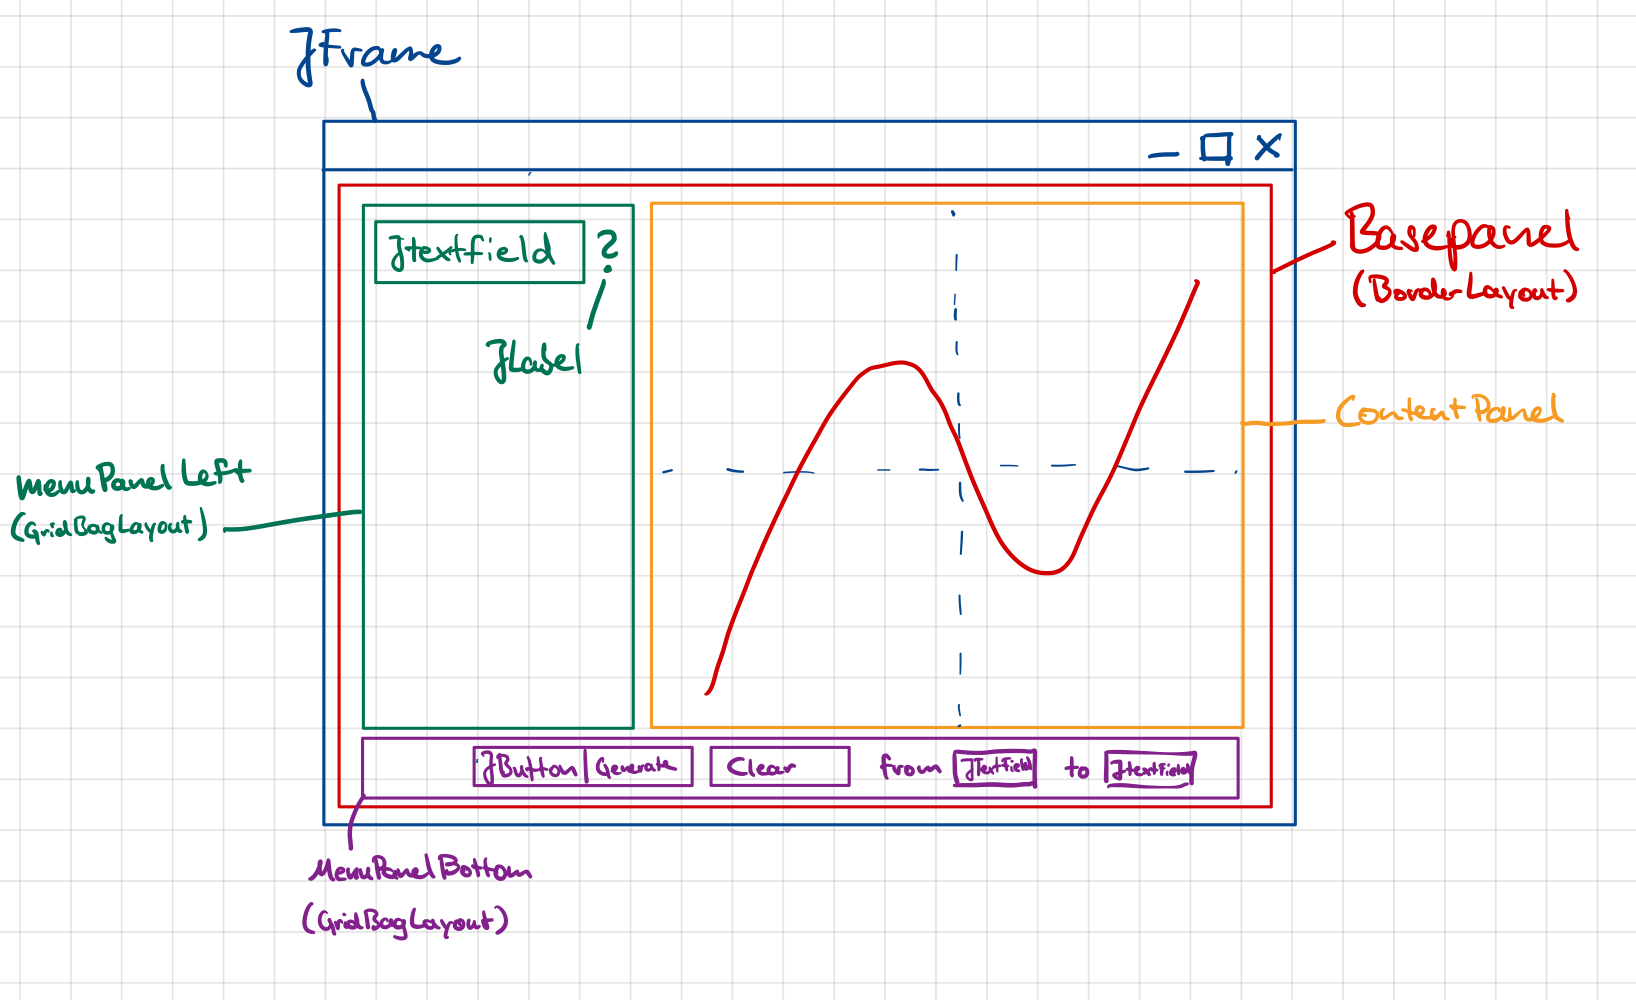
\includegraphics[scale=0.25]{images/sketch.png}
		\end{center}

		\caption{Entwurfsskizze}
	\end{figure}

\end{document}